% Seminar 4: Modele SARIMA
% Prezentare academică de calitate Harvard
% Program de licență, Academia de Studii Economice din București

\documentclass[9pt, aspectratio=169, t]{beamer}

% Asigură încadrarea conținutului pe diapozitive
\setbeamersize{text margin left=8mm, text margin right=8mm}

%=============================================================================
% CONFIGURARE TEMĂ ȘI STIL
%=============================================================================
\usetheme{default}

% Color Palette (matching Redispatch PDF)
\definecolor{MainBlue}{RGB}{26, 58, 110}
\definecolor{AccentBlue}{RGB}{26, 58, 110}
\definecolor{IDAred}{RGB}{205, 0, 0}
\definecolor{DarkGray}{RGB}{51, 51, 51}
\definecolor{MediumGray}{RGB}{128, 128, 128}
\definecolor{LightGray}{RGB}{248, 248, 248}
\definecolor{VeryLightGray}{RGB}{235, 235, 235}
\definecolor{KeynoteGray}{RGB}{218, 218, 218}
\definecolor{SectionGray}{RGB}{120, 120, 120}
\definecolor{FooterGray}{RGB}{100, 100, 100}
\definecolor{Crimson}{RGB}{220, 53, 69}
\definecolor{Forest}{RGB}{46, 125, 50}
\definecolor{Amber}{RGB}{181, 133, 63}
\definecolor{Orange}{RGB}{230, 126, 34}
\definecolor{Purple}{RGB}{142, 68, 173}

% Gradient background (exact Keynote 315 gradient: white to RGB 218,218,218)
\setbeamertemplate{background}{%
    \begin{tikzpicture}[remember picture, overlay]
        \shade[shading=axis, shading angle=315,
        top color=white, bottom color=KeynoteGray]
        (current page.south west) rectangle (current page.north east);
    \end{tikzpicture}%
}
% Fallback solid color for compatibility
\setbeamercolor{background canvas}{bg=}

\setbeamercolor{palette primary}{bg=MainBlue, fg=white}
\setbeamercolor{palette secondary}{bg=MainBlue!85, fg=white}
\setbeamercolor{palette tertiary}{bg=MainBlue!70, fg=white}
\setbeamercolor{structure}{fg=MainBlue}
\setbeamercolor{title}{fg=IDAred}
\setbeamercolor{frametitle}{fg=IDAred, bg=}
\setbeamercolor{block title}{bg=MainBlue, fg=white}
\setbeamercolor{block body}{bg=VeryLightGray, fg=DarkGray}
\setbeamercolor{block title alerted}{bg=Crimson, fg=white}
\setbeamercolor{block body alerted}{bg=Crimson!8, fg=DarkGray}
\setbeamercolor{block title example}{bg=Forest, fg=white}
\setbeamercolor{block body example}{bg=Forest!8, fg=DarkGray}
\setbeamercolor{item}{fg=MainBlue}

% Footer colors (override Madrid theme blue)
\setbeamercolor{author in head/foot}{fg=FooterGray, bg=}
\setbeamercolor{title in head/foot}{fg=FooterGray, bg=}
\setbeamercolor{date in head/foot}{fg=FooterGray, bg=}
\setbeamercolor{section in head/foot}{fg=FooterGray, bg=}
\setbeamercolor{subsection in head/foot}{fg=FooterGray, bg=}

% Bullet styles (apply everywhere including blocks)
\setbeamertemplate{itemize item}{\color{MainBlue}$\boxdot$}
\setbeamertemplate{itemize subitem}{\color{MainBlue}$\blacktriangleright$}
\setbeamertemplate{itemize subsubitem}{\color{MainBlue}\tiny$\bullet$}
\setbeamertemplate{itemize/enumerate body begin}{\normalsize}
\setbeamertemplate{itemize/enumerate subbody begin}{\normalsize}

% Item spacing - compact style
\setlength{\leftmargini}{10pt}       % Level 1: minimal indent
\setlength{\leftmarginii}{10pt}      % Level 2: minimal additional indent
% Compact list spacing (zero extra space before/after lists in blocks)
\makeatletter
\def\@listi{\leftmargin\leftmargini \topsep 0pt \parsep 0pt \itemsep 0pt}
\def\@listii{\leftmargin\leftmarginii \topsep 0pt \parsep 0pt \itemsep 0pt}
\makeatother

\setbeamertemplate{navigation symbols}{}

%=============================================================================
% CUSTOM HEADLINE
%=============================================================================
\setbeamertemplate{headline}{%
    \vskip10pt%
    \hbox to \paperwidth{%
        \hskip0.5cm%
        {\small\color{FooterGray}\renewcommand{\hyperlink}[2]{##2}\insertsectionhead}%
        \hfill%
        \textcolor{FooterGray}{\small\insertframenumber}%
        \hskip0.5cm%
    }%
    \vskip4pt%
    {\color{FooterGray}\hrule height 0.4pt}%
}

%=============================================================================
% CUSTOM FOOTER
%=============================================================================
\usepackage{fontawesome5}

\setbeamertemplate{footline}{%
    {\color{FooterGray}\hrule height 0.4pt}%
    \vskip4pt%
    \hbox to \paperwidth{%
        \hskip0.5cm%
        \textcolor{FooterGray}{\small Analiza și Prognoza seriilor de timp}%
        \hfill%
        \raisebox{-0.1em}{%
            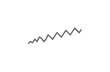
\begin{tikzpicture}[x=0.08em, y=0.08em, line width=0.4pt]
                \draw[FooterGray] (0,3) -- (1,4) -- (2,3.5) -- (3,5) -- (4,4) -- (5,6) -- (6,5.5) -- (7,4) -- (8,5) -- (9,7) -- (10,6) -- (11,5) -- (12,6.5) -- (13,8) -- (14,7) -- (15,6) -- (16,7.5) -- (17,9) -- (18,8) -- (19,7) -- (20,8.5) -- (21,10) -- (22,9) -- (23,8) -- (24,9.5);
            \end{tikzpicture}%
        }%
        \hskip0.5cm%
    }%
    \vskip6pt%
}

%=============================================================================
% PACHETE
%=============================================================================
\usepackage[utf8]{inputenc}
\usepackage[T1]{fontenc}
\usepackage[romanian]{babel}
\usepackage{amsmath, amssymb, amsthm}
\usepackage{mathtools}
\usepackage{bm}
\usepackage{tikz}
\usetikzlibrary{arrows.meta, positioning, shapes, calc, decorations.pathreplacing, shadings}
\usepackage{booktabs}
\usepackage{multirow}
\usepackage{array}
\usepackage{graphicx}
\usepackage{hyperref}
\usepackage{colortbl}
\hypersetup{colorlinks=true, linkcolor=MainBlue, urlcolor=MainBlue}
\graphicspath{{../../logos/}{../../charts/}}
\hfuzz=2pt  % Suppress tiny overfull warnings (<2pt)
\vfuzz=2pt  % Suppress tiny vertical overfull warnings (<2pt)

%=============================================================================
% COMANDA QUANTLET
%=============================================================================
\newcommand{\quantlet}[2]{%
    \hfill\href{#2}{%
        \raisebox{-0.15em}{\includegraphics[height=0.7em]{ql_logo.png}}%
        \textcolor{MainBlue}{\tiny\ #1}%
    }%
}

%=============================================================================
%=============================================================================
% CENTRED MINIPAGE (fara spatiu vertical suplimentar)
%=============================================================================
\newenvironment{cminipage}[1]{%
    \par\noindent\hfill\begin{minipage}{#1}\ignorespaces
}{%
    \end{minipage}\hfill\null\par
}


% COMENZI PERSONALIZATE
%=============================================================================
\newcommand{\E}{\mathbb{E}}
\newcommand{\Var}{\text{Var}}
\newcommand{\Cov}{\text{Cov}}
\newcommand{\Corr}{\text{Corr}}
\newcommand{\R}{\mathbb{R}}
\newcommand{\RMSE}{\text{RMSE}}
\newcommand{\MAE}{\text{MAE}}
\newcommand{\MAPE}{\text{MAPE}}

\newcommand{\correct}{\textcolor{Forest}{\checkmark}}
\newcommand{\incorrect}{\textcolor{Crimson}{\texttimes}}

%=============================================================================
% PAGINA TITLU PERSONALIZATA
%=============================================================================
\defbeamertemplate*{title page}{hybrid}[1][]
{
    \vspace{0.2cm}
    \begin{center}
        \href{https://www.ase.ro}{\includegraphics[height=1.0cm]{ase_logo.png}}\hspace{0.3cm}%
        \href{https://theida.net}{\includegraphics[height=1.0cm]{ida_logo.png}}\hspace{0.3cm}%
        \href{https://blockchain-research-center.com}{\includegraphics[height=1.0cm]{brc_logo.png}}\hspace{0.3cm}%
        \href{https://www.ai4efin.ase.ro}{\includegraphics[height=1.0cm]{ai4efin_logo.png}}\hspace{0.3cm}%
        \href{https://ipe.ro/new}{\includegraphics[height=1.0cm]{acad_logo.png}}\hspace{0.3cm}%
        \href{https://www.digital-finance-msca.com}{\includegraphics[height=1.0cm]{msca_logo.png}}%
    \end{center}

    \vspace{0.6cm}

    \begin{center}
        \begin{minipage}{0.1\textwidth}
            \centering
            \href{https://quantlet.com}{\includegraphics[height=1.1cm]{ql_logo.png}}
        \end{minipage}%
        \begin{minipage}{0.78\textwidth}
            \centering
            {\LARGE\bfseries\usebeamercolor[fg]{title}\inserttitle}

            \vspace{0.3cm}

            {\usebeamerfont{subtitle}\usebeamercolor[fg]{title}\insertsubtitle}
        \end{minipage}%
        \begin{minipage}{0.1\textwidth}
            \centering
            \href{https://quantinar.com}{\includegraphics[height=1.1cm]{qr_logo.png}}
        \end{minipage}
    \end{center}

    \vspace{0.6cm}

    \hspace{0.5cm}{\usebeamerfont{author}\insertauthor}

    \vspace{0.3cm}

    \hspace{0.5cm}\begin{minipage}[t]{0.9\textwidth}
        \raggedright\small\insertinstitute
    \end{minipage}
}

%=============================================================================
% INFORMATII TITLU
%=============================================================================
\title[Analiza Seriilor de Timp]{Analiza și Prognoza seriilor de timp}
\subtitle{Seminar 4: Modele SARIMA}
\author[D.T. Pele]{Daniel Traian PELE}
\institute{Academia de Studii Economice din București\\
IDA Institute Digital Assets\\
Blockchain Research Center\\
AI4EFin Artificial Intelligence for Energy Finance\\
Academia Română, Institutul de Prognoză Economică\\
MSCA Digital Finance}
\date{}

\begin{document}

% Title page (no header/footer)
{
\setbeamertemplate{headline}{}
\setbeamertemplate{footline}{}
\begin{frame}
    \titlepage
\end{frame}
}

%=============================================================================
% OUTLINE
%=============================================================================
\section{Prezentare Generală}

\begin{frame}{Cuprins Seminar}
    \begin{cminipage}{0.95\textwidth}
    \textbf{\large Structura seminarului:}

    \vspace{0.3cm}

    \begin{enumerate}
        \item[\textcolor{MainBlue}{\textbf{1.}}] \textbf{Prezentare Generală} -- Rezumatul conceptelor cheie
        \vspace{0.1cm}
        \item[\textcolor{MainBlue}{\textbf{2.}}] \textbf{Test de Recapitulare} -- Verificarea cunoștințelor
        \vspace{0.1cm}
        \item[\textcolor{MainBlue}{\textbf{3.}}] \textbf{Întrebări Adevărat/Fals} -- Verificări conceptuale
        \vspace{0.1cm}
        \item[\textcolor{MainBlue}{\textbf{4.}}] \textbf{Probleme Practice} -- Practică aplicată
        \vspace{0.1cm}
        \item[\textcolor{MainBlue}{\textbf{5.}}] \textbf{Exemple Rezolvate} -- Soluții detaliate
        \vspace{0.1cm}
        \item[\textcolor{MainBlue}{\textbf{6.}}] \textbf{Analiză pe Date Reale} -- Aplicații empirice
        \vspace{0.1cm}
        \item[\textcolor{MainBlue}{\textbf{7.}}] \textbf{Subiecte de Discuție} -- Gândire critică
        \vspace{0.1cm}
        \item[\textcolor{MainBlue}{\textbf{8.}}] \textbf{Rezumat} -- Sinteză finală
        \vspace{0.1cm}
        \item[\textcolor{MainBlue}{\textbf{9.}}] \textbf{Exerciții AI} -- Inteligență artificială aplicată
        \vspace{0.1cm}
        \item[\textcolor{MainBlue}{\textbf{10.}}] \textbf{Formule cheie} -- Referință rapidă
    \end{enumerate}
    \end{cminipage}
\end{frame}

%=============================================================================
% SECTION 1: REVIEW QUIZ
%=============================================================================
\section{Test de Recapitulare}

\begin{frame}{Test 1: Diferențierea Sezonieră}
    \begin{cminipage}{0.95\textwidth}
    \begin{alertblock}{Întrebare}
        Pentru date lunare cu sezonalitate anuală, ce face operatorul $(1-L^{12})$?
    \end{alertblock}

    \vspace{0.1cm}

    \begin{block}{Variante de răspuns}
        \textcolor{MainBlue}{\textbf{(A)}} Ia 12 diferențe consecutive \qquad
{indent}    \textcolor{MainBlue}{\textbf{(B)}} Calculează $Y_t - Y_{t-12}$ \qquad
{indent}    \textcolor{MainBlue}{\textbf{(C)}} Face media pe 12 luni \qquad
{indent}    \textcolor{MainBlue}{\textbf{(D)}} Elimină primele 12 observații
    \end{block}

    \vspace{0.3cm}
    \pause
    \begin{exampleblock}{Răspuns: B -- Calculează $Y_t - Y_{t-12}$}
        {\small
        \textbf{Operatorul de diferență sezonieră}:
        \vspace{-0.2cm}
        \[
        (1-L^{12})Y_t = Y_t - L^{12}Y_t = Y_t - Y_{t-12}
        \]
        \vspace{-0.3cm}

        \textbf{Exemplu} (vânzări ianuarie): $Y_{Ian2025} - Y_{Ian2024}$

        \textbf{Efect}: Elimină modelul sezonier anual stabil

        \textbf{Notă}: $(1-L^s)$ pentru orice perioadă sezonieră $s$ (trimestrial: $s=4$, săptămânal: $s=52$)
        }
    \end{exampleblock}
    \end{cminipage}
\end{frame}

\begin{frame}{Vizual: Diferența Sezonieră}
    \begin{cminipage}{0.95\textwidth}
    \begin{center}
        \includegraphics[width=0.95\textwidth]{ch4_def_seasonal_diff.pdf}
    \end{center}
    \vspace{-0.2cm}
    \small Diferențierea sezonieră elimină modelele anuale comparând aceleași perioade între ani.
    \quantlet{TSA\_ch4\_def\_seasonal\_diff}{https://github.com/QuantLet/TSA/tree/main/TSA_ch4/TSA_ch4_def_seasonal_diff}
    \end{cminipage}
\end{frame}

\begin{frame}{Test 2: Notația SARIMA}
    \begin{cminipage}{0.95\textwidth}
    \begin{alertblock}{Întrebare}
        Ce reprezintă SARIMA$(1,1,1) \times (1,1,1)_{12}$?
    \end{alertblock}

    \vspace{0.3cm}

    \begin{block}{Variante de răspuns}
        \textcolor{MainBlue}{\textbf{(A)}} 12 modele ARIMA diferite\\[3pt]
        \textcolor{MainBlue}{\textbf{(B)}} ARIMA cu 12 termeni AR și 12 termeni MA\\[3pt]
        \textcolor{MainBlue}{\textbf{(C)}} ARIMA(1,1,1) cu ARIMA(1,1,1) sezonier la perioada 12\\[3pt]
        \textcolor{MainBlue}{\textbf{(D)}} Un model care necesită 12 ani de date
    \end{block}
    \end{cminipage}
\end{frame}

\begin{frame}{Test 2: Răspuns}
    \begin{cminipage}{0.95\textwidth}
    \begin{exampleblock}{Răspuns: C -- ARIMA(1,1,1) cu ARIMA(1,1,1) sezonier la perioada 12}
        \begin{center}
            \includegraphics[width=0.95\textwidth, height=0.55\textheight, keepaspectratio]{sem4_sarima_notation.pdf}
        \end{center}
        $(1-\phi_1 L)(1-\Phi_1 L^{12})(1-L)(1-L^{12})Y_t = (1+\theta_1 L)(1+\Theta_1 L^{12})\varepsilon_t$
    \end{exampleblock}
    \end{cminipage}
\end{frame}

\begin{frame}{Vizual: Structura Modelului SARIMA}
    \begin{cminipage}{0.95\textwidth}
    \begin{center}
        \includegraphics[width=0.95\textwidth, height=0.78\textheight, keepaspectratio]{ch4_def_sarima.pdf}
    \end{center}
    \vspace{-0.2cm}
    \small SARIMA combină componentele ARIMA obișnuite cu componentele sezoniere la lag-ul $s$.
    \quantlet{TSA\_ch4\_def\_sarima}{https://github.com/QuantLet/TSA/tree/main/TSA_ch4/TSA_ch4_def_sarima}
    \end{cminipage}
\end{frame}

\begin{frame}{Test 3: Modelul Airline}
    \begin{cminipage}{0.95\textwidth}
    \begin{alertblock}{Întrebare}
        ``Modelul airline'' se referă la SARIMA$(0,1,1) \times (0,1,1)_{12}$. Câți parametri are (excluzând varianța)?
    \end{alertblock}

    \vspace{0.3cm}

    \begin{block}{Variante de răspuns}
        \textcolor{MainBlue}{\textbf{(A)}} 2 parametri \qquad
{indent}    \textcolor{MainBlue}{\textbf{(B)}} 4 parametri \qquad
{indent}    \textcolor{MainBlue}{\textbf{(C)}} 6 parametri \qquad
{indent}    \textcolor{MainBlue}{\textbf{(D)}} 12 parametri
    \end{block}
    \end{cminipage}
\end{frame}

\begin{frame}{Test 3: Răspuns}
    \begin{cminipage}{0.95\textwidth}
    \begin{exampleblock}{Răspuns: A -- 2 parametri ($\theta_1$ și $\Theta_1$)}
        \begin{center}
            \includegraphics[width=0.95\textwidth, height=0.55\textheight, keepaspectratio]{sem4_airline_model.pdf}
        \end{center}
        \textbf{Modelul airline}: $(1-L)(1-L^{12})Y_t = (1+\theta_1 L)(1+\Theta_1 L^{12})\varepsilon_t$

        Se potrivește remarcabil de bine pe multe serii economice sezoniere (Box \& Jenkins, 1970)
    \end{exampleblock}
    \end{cminipage}
\end{frame}

\begin{frame}{Test 4: ACF-ul Datelor Sezoniere}
    \begin{cminipage}{0.95\textwidth}
    \begin{alertblock}{Întrebare}
        Pentru date lunare cu sezonalitate puternică, unde vă așteptați să vedeți vârfuri ACF semnificative?
    \end{alertblock}

    \vspace{0.3cm}

    \begin{block}{Variante de răspuns}
        \textcolor{MainBlue}{\textbf{(A)}} Doar la lag 1 \qquad
{indent}    \textcolor{MainBlue}{\textbf{(B)}} Doar la lag 12 \qquad
{indent}    \textcolor{MainBlue}{\textbf{(C)}} La lag-urile 12, 24, 36, ... \qquad
{indent}    \textcolor{MainBlue}{\textbf{(D)}} Distribuite aleatoriu
    \end{block}

    \vspace{0.5cm}
    \pause
    \begin{exampleblock}{Răspuns: C -- La lag-urile 12, 24, 36, ...}
        {\small
        \textbf{Intuiție}: Ianuarie 2024 este similar cu ianuarie 2023, 2022, etc.

        \textbf{Model ACF}: Vârfuri la lag-urile $s, 2s, 3s, \ldots$ ($\rho_{12}, \rho_{24}, \rho_{36} \neq 0$)

        \textbf{Diagnostic}: Descreștere lentă la lag-urile sezoniere $\Rightarrow$ $D=1$; Întrerupere după lag $s$ $\Rightarrow$ $Q=1$
        }
    \end{exampleblock}
    \end{cminipage}
\end{frame}

\begin{frame}{Vizual: Modele de Sezonalitate}
    \begin{cminipage}{0.95\textwidth}
    \begin{center}
        \includegraphics[width=0.95\textwidth]{ch4_def_seasonality.pdf}
    \end{center}
    \vspace{-0.2cm}
    \small Modelele sezoniere se repetă la intervale regulate (lunar, trimestrial, etc.) și pot fi aditive sau multiplicative.
    \quantlet{TSA\_ch4\_def\_seasonality}{https://github.com/QuantLet/TSA/tree/main/TSA_ch4/TSA_ch4_def_seasonality}
    \end{cminipage}
\end{frame}

\begin{frame}{Test 5: Structura Multiplicativă}
    \vspace{-0.5cm}
    \begin{cminipage}{0.95\textwidth}
    \begin{alertblock}{Întrebare}
        În SARIMA, ce înseamnă ``structură multiplicativă''?
    \end{alertblock}

    \vspace{0.1cm}

    \begin{block}{Variante de răspuns}
        \textcolor{MainBlue}{\textbf{(A)}} Amplitudinea sezonieră crește proporțional\\[3pt]
        \textcolor{MainBlue}{\textbf{(B)}} Polinoamele obișnuite și sezoniere sunt înmulțite\\[3pt]
        \textcolor{MainBlue}{\textbf{(C)}} Înmulțim datele cu factori sezonieri\\[3pt]
        \textcolor{MainBlue}{\textbf{(D)}} Modelul este estimat folosind înmulțirea
    \end{block}

    \vspace{0.1cm}
    \pause
    \begin{exampleblock}{Răspuns: B -- Polinoamele obișnuite și sezoniere sunt înmulțite}
        {\footnotesize
        \textbf{SARIMA multiplicativ}: $\phi(L)\Phi(L^s)(1-L)^d(1-L^s)^D Y_t = \theta(L)\Theta(L^s)\varepsilon_t$

        \textbf{Exemplu}: $(1-\phi_1 L)(1-\Phi_1 L^{12}) = 1 - \phi_1 L - \Phi_1 L^{12} + \phi_1\Phi_1 L^{13}$

        \textbf{Termenul încrucișat} $\phi_1\Phi_1 L^{13}$: Captează interacțiunea între dinamica pe termen scurt și lung
        }
    \end{exampleblock}
    \end{cminipage}
\end{frame}

\begin{frame}{Test 6: Diferențierea Sezonieră vs Obișnuită}
    \vspace{-0.5cm}
    \begin{cminipage}{0.95\textwidth}
    \begin{alertblock}{Întrebare}
        Când ați aplica atât diferențierea obișnuită ($d=1$) cât și sezonieră ($D=1$)?
    \end{alertblock}

    \vspace{0.1cm}

    \begin{block}{Variante de răspuns}
        \textcolor{MainBlue}{\textbf{(A)}} Când datele au doar un trend\\[3pt]
        \textcolor{MainBlue}{\textbf{(B)}} Când datele au doar sezonalitate\\[3pt]
        \textcolor{MainBlue}{\textbf{(C)}} Când datele au atât trend cât și nestaționaritate sezonieră\\[3pt]
        \textcolor{MainBlue}{\textbf{(D)}} Niciodată -- se anulează reciproc
    \end{block}

    \vspace{0.1cm}
    \pause
    \begin{exampleblock}{Răspuns: C -- Atât trend cât și nestaționaritate sezonieră}
        {\footnotesize
        \textbf{Combinat}: $W_t = (1-L)(1-L^{12})Y_t = Y_t - Y_{t-1} - Y_{t-12} + Y_{t-13}$

        \textbf{Când este necesar}: ACF cu descreștere lentă la lag-urile 1,2,3... $\Rightarrow d=1$; la lag-urile 12,24,36... $\Rightarrow D=1$

        \textbf{Exemple}: Pasageri aerieni, vânzări retail, cerere de energie
        }
    \end{exampleblock}
    \end{cminipage}
\end{frame}

\begin{frame}{Test 7: Detectarea Sezonalității din ACF}
    \begin{cminipage}{0.95\textwidth}
    \begin{alertblock}{Întrebare}
        ACF-ul unei serii de timp lunare arată descreștere lentă la lag-urile 12, 24 și 36. Ce sugerează aceasta?
    \end{alertblock}

    \vspace{0.3cm}

    \begin{block}{Variante de răspuns}
        \textcolor{MainBlue}{\textbf{(A)}} Seria este staționară\\[3pt]
        \textcolor{MainBlue}{\textbf{(B)}} Seria necesită doar diferențierea obișnuită\\[3pt]
        \textcolor{MainBlue}{\textbf{(C)}} Seria are o rădăcină unitară sezonieră necesitând $D=1$\\[3pt]
        \textcolor{MainBlue}{\textbf{(D)}} Seria este zgomot alb
    \end{block}
    \end{cminipage}
\end{frame}

\begin{frame}{Test 7: Răspuns}
    \begin{cminipage}{0.95\textwidth}
    \begin{exampleblock}{Răspuns: C -- Rădăcină unitară sezonieră necesitând $D=1$}
        \begin{center}
            \includegraphics[width=0.95\textwidth, height=0.55\textheight, keepaspectratio]{sem4_seasonal_acf.pdf}
        \end{center}
        \textbf{Stânga}: Sezonieră staționară (descreștere rapidă la lag-urile sezoniere)

        \textbf{Dreapta}: Rădăcină unitară sezonieră (descreștere lentă $\Rightarrow$ necesită $D=1$)
    \end{exampleblock}
    \end{cminipage}
\end{frame}

\begin{frame}{Test 8: Sezonalitate Multiplicativă vs Aditivă}
    \begin{cminipage}{0.95\textwidth}
    \begin{alertblock}{Întrebare}
        Dacă amplitudinea sezonieră a unei serii de timp crește proporțional cu nivelul, aceasta indică:
    \end{alertblock}

    \vspace{0.3cm}

    \begin{block}{Variante de răspuns}
        \textcolor{MainBlue}{\textbf{(A)}} Sezonalitate aditivă -- folosiți $(1-L^s)$\\[3pt]
        \textcolor{MainBlue}{\textbf{(B)}} Sezonalitate multiplicativă -- folosiți transformarea $\log$\\[3pt]
        \textcolor{MainBlue}{\textbf{(C)}} Fără sezonalitate prezentă\\[3pt]
        \textcolor{MainBlue}{\textbf{(D)}} Nevoie doar de diferențiere obișnuită
    \end{block}
    \end{cminipage}
\end{frame}

\begin{frame}{Test 8: Răspuns}
    \begin{cminipage}{0.95\textwidth}
    \begin{exampleblock}{Răspuns: B -- Sezonalitate multiplicativă, folosiți transformarea $\log$}
        \begin{center}
            \includegraphics[width=0.95\textwidth, height=0.55\textheight, keepaspectratio]{sem4_mult_add.pdf}
        \end{center}
        \textbf{Multiplicativă}: Amplitudinea sezonieră crește cu nivelul (linii divergente)

        \textbf{Soluție}: Aplicați transformarea $\log$ înainte de a ajusta SARIMA
    \end{exampleblock}
    \end{cminipage}
\end{frame}

\begin{frame}{Test 9: Graficul Subseriilor Sezoniere}
    \vspace{-0.5cm}
    \begin{cminipage}{0.95\textwidth}
    \begin{alertblock}{Întrebare}
        Într-un grafic de subserii sezoniere, ce indică sezonalitatea multiplicativă?
    \end{alertblock}

    \vspace{0.1cm}

    \begin{block}{Variante de răspuns}
        \textcolor{MainBlue}{\textbf{(A)}} Liniile pentru fiecare lună sunt paralele\\[3pt]
        \textcolor{MainBlue}{\textbf{(B)}} Liniile pentru fiecare lună divergează (dispersia crește în timp)\\[3pt]
        \textcolor{MainBlue}{\textbf{(C)}} Toate lunile au aceeași medie\\[3pt]
        \textcolor{MainBlue}{\textbf{(D)}} Liniile sunt orizontale
    \end{block}

    \vspace{0.1cm}
    \pause
    \begin{exampleblock}{Răspuns: B -- Liniile divergează (dispersia crește în timp)}
        {\footnotesize
        \textbf{Graficul subseriilor}: Grupează datele pe luni, reprezintă valorile fiecărei luni de-a lungul anilor

        \textbf{Paralele} $\Rightarrow$ Aditivă; \textbf{Divergente} $\Rightarrow$ Multiplicativă; \textbf{Orizontale} $\Rightarrow$ Fără trend

        \textbf{Acțiune}: Dacă multiplicativă, aplicați $\log$ înainte de a ajusta SARIMA
        }
    \end{exampleblock}
    \end{cminipage}
\end{frame}

\begin{frame}{Test 10: Invertibilitatea în SARIMA}
    \vspace{-0.5cm}
    \begin{cminipage}{0.95\textwidth}
    \begin{alertblock}{Întrebare}
        Pentru ca SARIMA$(0,1,1) \times (0,1,1)_{12}$ să fie invertibil, care condiție trebuie îndeplinită?
    \end{alertblock}

    \vspace{0.1cm}

    \begin{block}{Variante de răspuns}
        \textcolor{MainBlue}{\textbf{(A)}} $|\theta_1| < 1$ doar\\[3pt]
        \textcolor{MainBlue}{\textbf{(B)}} $|\Theta_1| < 1$ doar\\[3pt]
        \textcolor{MainBlue}{\textbf{(C)}} Atât $|\theta_1| < 1$ cât și $|\Theta_1| < 1$\\[3pt]
        \textcolor{MainBlue}{\textbf{(D)}} Nu există condiție de invertibilitate pentru modelele MA
    \end{block}

    \vspace{0.1cm}
    \pause
    \begin{exampleblock}{Răspuns: C -- Atât $|\theta_1| < 1$ cât și $|\Theta_1| < 1$}
        {\scriptsize
        \textbf{Invertibilitate}: Toate rădăcinile MA în afara cercului unitate

        \textbf{MA multiplicativ}: $(1+\theta_1 L)(1+\Theta_1 L^{12})$

        \textbf{Rădăcini}: Obișnuită $|z| = |{-1}/{\theta_1}| > 1 \Leftrightarrow |\theta_1| < 1$; Sezonieră $|\Theta_1| < 1$

        \textbf{Ambele} condiții necesare pentru invertibilitate generală!
        }
    \end{exampleblock}
    \end{cminipage}
\end{frame}

\begin{frame}{Test 11: Testul HEGY}
    \vspace{-0.5cm}
    \begin{cminipage}{0.95\textwidth}
    \begin{alertblock}{Întrebare}
        Testul HEGY este folosit pentru:
    \end{alertblock}

    \vspace{0.1cm}

    \begin{block}{Variante de răspuns}
        \textcolor{MainBlue}{\textbf{(A)}} Estimarea parametrilor SARIMA\\[3pt]
        \textcolor{MainBlue}{\textbf{(B)}} Testarea rădăcinilor unitare la diferite frecvențe (trend și sezoniere)\\[3pt]
        \textcolor{MainBlue}{\textbf{(C)}} Verificarea normalității reziduurilor\\[3pt]
        \textcolor{MainBlue}{\textbf{(D)}} Compararea modelelor SARIMA folosind criterii informaționale
    \end{block}

    \vspace{0.1cm}
    \pause
    \begin{exampleblock}{Răspuns: B -- Testarea rădăcinilor unitare la diferite frecvențe}
        {\footnotesize
        \textbf{Testul HEGY} (Hylleberg-Engle-Granger-Yoo, 1990):

        Testează la: Frecvența zero ($\omega = 0$) $\Rightarrow d = 1$; Nyquist ($\omega = \pi$); Sezonieră $\Rightarrow D = 1$

        \textbf{Decizie}: Respingeți toate $\Rightarrow$ variabile dummy sezoniere; Nu respingeți sezoniera $\Rightarrow$ diferențiere sezonieră
        }
    \end{exampleblock}
    \end{cminipage}
\end{frame}

\begin{frame}{Test 12: Identificarea MA Sezonier}
    \vspace{-0.5cm}
    \begin{cminipage}{0.95\textwidth}
    \begin{alertblock}{Întrebare}
        După aplicarea $(1-L)(1-L^{12})$, ACF arată un singur vârf semnificativ doar la lag 12 (fără vârf la lag 1). PACF descrește la lag-urile sezoniere. Aceasta sugerează:
    \end{alertblock}

    \vspace{0.1cm}

    \begin{block}{Variante de răspuns}
        \textcolor{MainBlue}{\textbf{(A)}} SARIMA$(0,1,0) \times (0,1,1)_{12}$\\[3pt]
        \textcolor{MainBlue}{\textbf{(B)}} SARIMA$(0,1,1) \times (0,1,0)_{12}$\\[3pt]
        \textcolor{MainBlue}{\textbf{(C)}} SARIMA$(1,1,0) \times (1,1,0)_{12}$\\[3pt]
        \textcolor{MainBlue}{\textbf{(D)}} SARIMA$(0,1,1) \times (0,1,1)_{12}$
    \end{block}

    \vspace{0.1cm}
    \pause
    \begin{exampleblock}{Răspuns: A -- SARIMA$(0,1,0) \times (0,1,1)_{12}$}
        {\scriptsize
        \textbf{Model}: Lag-uri obișnuite -- fără vârfuri în ACF/PACF; Lag-uri sezoniere -- ACF se anulează la $s$, PACF descrește

        \textbf{Interpretare}: Fără MA obișnuit ($q = 0$); MA(1) sezonier indicat ($Q = 1$)

        \textbf{Model}: $(1-L)(1-L^{12})Y_t = (1 + \Theta_1 L^{12})\varepsilon_t$
        }
    \end{exampleblock}
    \end{cminipage}
\end{frame}

\begin{frame}{Test 13: Supradiferențierea}
    \vspace{-0.5cm}
    \begin{cminipage}{0.95\textwidth}
    \begin{alertblock}{Întrebare}
        După diferențiere, ACF arată un vârf negativ mare la lag 1 sau lag $s$. Aceasta indică de obicei:
    \end{alertblock}

    \vspace{0.1cm}

    \begin{block}{Variante de răspuns}
        \textcolor{MainBlue}{\textbf{(A)}} Modelul necesită mai mulți termeni AR\\[3pt]
        \textcolor{MainBlue}{\textbf{(B)}} Seria a fost supradiferențiată\\[3pt]
        \textcolor{MainBlue}{\textbf{(C)}} Seria este perfect staționară\\[3pt]
        \textcolor{MainBlue}{\textbf{(D)}} Prezența heteroscedasticității
    \end{block}

    \vspace{0.1cm}
    \pause
    \begin{exampleblock}{Răspuns: B -- Seria a fost supradiferențiată}
        {\footnotesize
        \textbf{Semnătură}: ACF la lag 1 $\approx -0.5$ $\Rightarrow$ supradif la $d$; ACF la lag $s$ $\approx -0.5$ $\Rightarrow$ supradif la $D$

        \textbf{De ce?} $\Delta^2 Y_t = \varepsilon_t - \varepsilon_{t-1}$ este MA(1) cu $\theta = -1$, dând $\rho_1 = -0.5$

        \textbf{Corecție}: Reduceți $d$ sau $D$ cu unu și re-examinați ACF/PACF
        }
    \end{exampleblock}
    \end{cminipage}
\end{frame}

\begin{frame}{Test 14: Orizontul de Prognoză}
    \begin{cminipage}{0.95\textwidth}
    \begin{alertblock}{Întrebare}
        Pentru un model SARIMA cu $D=1$, ce se întâmplă cu intervalele de încredere ale prognozei când orizontul $h \to \infty$?
    \end{alertblock}

    \vspace{0.3cm}

    \begin{block}{Variante de răspuns}
        \textcolor{MainBlue}{\textbf{(A)}} Converg la o lățime fixă \qquad
{indent}    \textcolor{MainBlue}{\textbf{(B)}} Cresc fără limită \qquad
{indent}    \textcolor{MainBlue}{\textbf{(C)}} Se micșorează la zero \qquad
{indent}    \textcolor{MainBlue}{\textbf{(D)}} Oscilează sezonier
    \end{block}

    \vspace{0.5cm}
    \pause
    \begin{exampleblock}{Răspuns: B -- Cresc fără limită}
        {\small
        \textbf{Proprietatea rădăcinii unitare}: Orice rădăcină unitară cauzează varianță de prognoză nemărginită

        \textbf{Pentru SARIMA cu $D=1$}: $\Var(\hat{Y}_{T+h} - Y_{T+h}) \to \infty$ când $h \to \infty$

        \textbf{Intuiție}: Șocurile sezoniere se acumulează; prognozele pe termen lung au IC-uri largi
        }
    \end{exampleblock}
    \end{cminipage}
\end{frame}

\begin{frame}{Test 15: Selectarea Perioadei Sezoniere}
    \begin{cminipage}{0.95\textwidth}
    \begin{alertblock}{Întrebare}
        Aveți date zilnice care arată modele săptămânale clare. Ce perioadă sezonieră $s$ ar trebui să folosiți într-un model SARIMA?
    \end{alertblock}

    \vspace{0.1cm}

    \begin{block}{Variante de răspuns}
        \textcolor{MainBlue}{\textbf{(A)}} $s = 12$ (lunar) \qquad
{indent}    \textcolor{MainBlue}{\textbf{(B)}} $s = 7$ (săptămânal) \qquad
{indent}    \textcolor{MainBlue}{\textbf{(C)}} $s = 365$ (anual) \qquad
{indent}    \textcolor{MainBlue}{\textbf{(D)}} $s = 24$ (orar)
    \end{block}

    \vspace{0.2cm}
    \pause
    \begin{exampleblock}{Răspuns: B -- $s = 7$ (săptămânal)}
        {\small
        \begin{center}
        \vspace{-0.2cm}
        \begin{tabular}{lll}
            \textbf{Date} & \textbf{Model} & \textbf{Perioada $s$} \\
            Zilnice & Săptămânal & 7 \\
            Lunare & Anual & 12 \\
            Trimestriale & Anual & 4
        \end{tabular}
        \end{center}
        \vspace{-0.1cm}
        \textbf{Regulă}: $s$ = observații per ciclu al modelului dominant
        }
    \end{exampleblock}
    \end{cminipage}
\end{frame}

\begin{frame}{Test 16: Componenta AR Sezonieră}
    \vspace{-0.5cm}
    \begin{cminipage}{0.95\textwidth}
    \begin{alertblock}{Întrebare}
        În componenta sezonieră $\Phi(L^s) = 1 - \Phi_1 L^s$, ce ne spune coeficientul $\Phi_1 = 0.8$?
    \end{alertblock}

    \vspace{0.1cm}

    \begin{block}{Variante de răspuns}
        \textcolor{MainBlue}{\textbf{(A)}} 80\% din valoarea perioadei curente vine din perioada anterioară\\[3pt]
        \textcolor{MainBlue}{\textbf{(B)}} Există 80\% corelație între observațiile consecutive\\[3pt]
        \textcolor{MainBlue}{\textbf{(C)}} 80\% din valoarea perioadei curente este explicată de aceeași perioadă din anul trecut\\[3pt]
        \textcolor{MainBlue}{\textbf{(D)}} Modelul sezonier explică 80\% din varianță
    \end{block}

    \vspace{0.1cm}
    \pause
    \begin{exampleblock}{Răspuns: C -- 80\% explicat de aceeași perioadă din anul trecut}
        {\scriptsize
        \textbf{SAR(1)}: $Y_t = \Phi_1 Y_{t-12} + \varepsilon_t$

        \textbf{Cu $\Phi_1 = 0.8$}: $Y_{Ian2024} = 0.8 \cdot Y_{Ian2023} + \varepsilon_t$

        \textbf{Interpretare}: Persistență sezonieră puternică -- 80\% explicat de aceeași lună din anul trecut

        \textbf{Staționaritate}: Necesită $|\Phi_1| < 1$ (satisfăcută aici)
        }
    \end{exampleblock}
    \end{cminipage}
\end{frame}

\begin{frame}{Test 17: Staționaritatea Sezonieră}
    \vspace{-0.5cm}
    \begin{cminipage}{0.95\textwidth}
    \begin{alertblock}{Întrebare}
        Un proces sezonier cu $\Phi_1 = 1$ în SARIMA$(0,0,0) \times (1,0,0)_{12}$ este:
    \end{alertblock}

    \vspace{0.1cm}

    \begin{block}{Variante de răspuns}
        \textcolor{MainBlue}{\textbf{(A)}} Staționar\\[3pt]
        \textcolor{MainBlue}{\textbf{(B)}} Are o rădăcină unitară sezonieră (integrat sezonier)\\[3pt]
        \textcolor{MainBlue}{\textbf{(C)}} Exploziv\\[3pt]
        \textcolor{MainBlue}{\textbf{(D)}} Nedefinit
    \end{block}

    \vspace{0.1cm}
    \pause
    \begin{exampleblock}{Răspuns: B -- Are o rădăcină unitară sezonieră}
        {\footnotesize
        \textbf{Model}: $Y_t = Y_{t-12} + \varepsilon_t$ (mers aleator sezonier)

        \textbf{Proprietăți}: Varianța crește cu timpul; fiecare lună urmează propriul său mers aleator; necesită $D = 1$

        \textbf{Analogie}: Ca mersul aleatoriu obișnuit dar la frecvența sezonieră
        }
    \end{exampleblock}
    \end{cminipage}
\end{frame}

\begin{frame}{Test 18: Compararea Modelelor}
    \vspace{-0.5cm}
    \begin{cminipage}{0.95\textwidth}
    \begin{alertblock}{Întrebare}
        Modelul A: SARIMA$(1,1,1) \times (1,1,1)_{12}$ are AIC = 520. Modelul B: SARIMA$(0,1,1) \times (0,1,1)_{12}$ are AIC = 525. Care afirmație este cea mai corectă?
    \end{alertblock}

    \vspace{0.1cm}

    \begin{block}{Variante de răspuns}
        \textcolor{MainBlue}{\textbf{(A)}} Modelul A este întotdeauna mai bun deoarece are AIC mai mic\\[3pt]
        \textcolor{MainBlue}{\textbf{(B)}} Modelul B ar trebui preferat datorită parcimoniei în ciuda AIC mai mare\\[3pt]
        \textcolor{MainBlue}{\textbf{(C)}} Diferența AIC de 5 sugerează că Modelul A este substanțial mai bun\\[3pt]
        \textcolor{MainBlue}{\textbf{(D)}} Nu putem compara modele cu ordine diferite
    \end{block}

    \vspace{0.1cm}
    \pause
    \begin{exampleblock}{Răspuns: C -- Diferența AIC de 5 sugerează că Modelul A este substanțial mai bun}
        {\scriptsize
        \textbf{Regulă empirică}: $\Delta$AIC $< 2$: echivalente; $2$--$10$: anumite dovezi; $> 10$: dovezi puternice

        \textbf{Aici}: $\Delta$AIC $= 5$ sugerează Modelul A semnificativ mai bun

        \textbf{Întotdeauna}: Verificați și diagnosticele reziduurilor și performanța prognozei!
        }
    \end{exampleblock}
    \end{cminipage}
\end{frame}

\begin{frame}{Test 19: Modele Sezoniere în Reziduuri}
    \vspace{-0.5cm}
    \begin{cminipage}{0.95\textwidth}
    \begin{alertblock}{Întrebare}
        După ajustarea unui model SARIMA, observați vârfuri ACF semnificative la lag-urile 12 și 24 în reziduuri. Ce indică aceasta?
    \end{alertblock}

    \vspace{0.1cm}

    \begin{block}{Variante de răspuns}
        \textcolor{MainBlue}{\textbf{(A)}} Modelul este corect specificat\\[3pt]
        \textcolor{MainBlue}{\textbf{(B)}} Componenta sezonieră este inadecvată\\[3pt]
        \textcolor{MainBlue}{\textbf{(C)}} Datele nu sunt sezoniere\\[3pt]
        \textcolor{MainBlue}{\textbf{(D)}} A apărut supraajustarea
    \end{block}

    \vspace{0.1cm}
    \pause
    \begin{exampleblock}{Răspuns: B -- Componenta sezonieră este inadecvată}
        {\scriptsize
        \textbf{Diagnostice}: Reziduurile bune ar trebui să fie zgomot alb (fără ACF semnificativ)

        \textbf{ACF sezonier în reziduuri}: Modelul nu a capturat structura sezonieră; încercați să creșteți $P$ sau $Q$; verificați că $D$ este corect

        \textbf{Acțiune}: Încercați SARIMA cu ordin sezonier mai mare, verificați Ljung-Box la lag-urile sezoniere
        }
    \end{exampleblock}
    \end{cminipage}
\end{frame}

\begin{frame}{Test 20: Prognoză Practică}
    \vspace{-0.5cm}
    \begin{cminipage}{0.95\textwidth}
    \begin{alertblock}{Întrebare}
        Prognozați vânzări retail lunare cu SARIMA$(0,1,1) \times (0,1,1)_{12}$. Pentru prognoza la 13 luni înainte, care observații istorice sunt cele mai influente?
    \end{alertblock}

    \vspace{0.1cm}

    \begin{block}{Variante de răspuns}
        \textcolor{MainBlue}{\textbf{(A)}} Doar cea mai recentă observație\\[3pt]
        \textcolor{MainBlue}{\textbf{(B)}} Observația de aceeași lună din anul trecut\\[3pt]
        \textcolor{MainBlue}{\textbf{(C)}} Toate observațiile în mod egal\\[3pt]
        \textcolor{MainBlue}{\textbf{(D)}} Doar observațiile din aceeași lună din toți anii anteriori
    \end{block}

    \vspace{0.1cm}
    \pause
    \begin{exampleblock}{Răspuns: B -- Observația de aceeași lună din anul trecut}
        {\footnotesize
        \textbf{Pentru 13 luni înainte}: Cea mai influentă este $Y_{T-11}$ (aceeași lună anul trecut), de asemenea $Y_T$ și $Y_{T-12}$

        \textbf{Intuiție}: ``Ianuarie viitor arată ca ianuarie trecut, ajustat pentru trendul recent''
        }
    \end{exampleblock}
    \end{cminipage}
\end{frame}

%=============================================================================
% TRUE/FALSE QUESTIONS
%=============================================================================
\section{Întrebări Adevărat/Fals}

\begin{frame}{Întrebări Adevărat/Fals (1-6)}
    \begin{cminipage}{0.95\textwidth}
    \begin{alertblock}{Întrebare}
        Determinați dacă fiecare afirmație este Adevărată sau Falsă:
    \end{alertblock}

    \vspace{0.3cm}
    {\small
    \begin{enumerate}
        \item Perioada sezonieră $s$ pentru date trimestriale cu modele anuale este $s=4$.
        \item Modelele SARIMA pot gestiona doar o singură frecvență sezonieră.
        \item Dacă AIC selectează SARIMA$(1,1,1) \times (1,1,1)_{12}$ și BIC selectează modelul airline, BIC greșește întotdeauna.
        \item Testul Kruskal-Wallis poate detecta sezonalitatea fără a presupune normalitate.
        \item După ajustarea unui model SARIMA, reziduurile nu ar trebui să arate ACF semnificativ la lag-urile sezoniere.
        \item Transformarea logaritmică convertește sezonalitatea multiplicativă în aditivă.
    \end{enumerate}
    }

    \vspace{0.3cm}
    \begin{center}
        \textit{Răspunsul pe slide-ul următor...}
    \end{center}
    \end{cminipage}
\end{frame}

\begin{frame}{Soluții Adevărat/Fals (1-6)}
    \begin{cminipage}{0.95\textwidth}
    \begin{exampleblock}{Răspunsuri}
    \begin{enumerate}
        \item \textcolor{Forest}{\textbf{ADEVĂRAT}}: Datele trimestriale cu ciclu anual au $s=4$ trimestre pe an.
        \item \textcolor{Forest}{\textbf{ADEVĂRAT}}: SARIMA standard gestionează un $s$; sezonalități multiple necesită TBATS sau termeni Fourier.
        \item \textcolor{Crimson}{\textbf{FALS}}: BIC penalizează complexitatea mai mult; modelul mai simplu poate fi mai bun pentru interpretare/prognoză.
        \item \textcolor{Forest}{\textbf{ADEVĂRAT}}: Kruskal-Wallis este neparametric, comparând distribuțiile între sezoane.
        \item \textcolor{Forest}{\textbf{ADEVĂRAT}}: ACF-ul reziduurilor ar trebui să fie în limitele de încredere la TOATE lag-urile inclusiv cele sezoniere.
        \item \textcolor{Forest}{\textbf{ADEVĂRAT}}: $\log(T \times S \times \varepsilon) = \log T + \log S + \log \varepsilon$ (formă aditivă).
    \end{enumerate}
    \end{exampleblock}
    \end{cminipage}
\end{frame}

%=============================================================================
% SECTION 2: PRACTICE PROBLEMS
%=============================================================================
\section{Probleme Practice}

\begin{frame}{Problema 1: Expandarea Diferenței Sezoniere}
    \begin{cminipage}{0.95\textwidth}
    \begin{block}{Exercițiu}
        Expandați complet $(1-L)(1-L^{12})Y_t$. Ce observații sunt implicate?
    \end{block}

    \vspace{0.3cm}
    \pause
    \begin{exampleblock}{Soluție}
        $(1-L)(1-L^{12}) = 1 - L - L^{12} + L^{13}$

        \vspace{0.2cm}
        Prin urmare:
        $(1-L)(1-L^{12})Y_t = Y_t - Y_{t-1} - Y_{t-12} + Y_{t-13}$

        \vspace{0.2cm}
        \textbf{Interpretare}: Aceasta este diferența diferențelor:
        \begin{itemize}
            \item Mai întâi diferența sezonieră: $Y_t - Y_{t-12}$ (anul acesta vs anul trecut)
            \item Apoi diferența obișnuită: $(Y_t - Y_{t-12}) - (Y_{t-1} - Y_{t-13})$
        \end{itemize}
    \end{exampleblock}
    \end{cminipage}
\end{frame}

\begin{frame}{Problema 2: Expandarea Modelului Airline}
    \begin{cminipage}{0.95\textwidth}
    \begin{block}{Exercițiu}
        Scrieți ecuația completă pentru modelul airline SARIMA$(0,1,1) \times (0,1,1)_{12}$:
        $(1-L)(1-L^{12})Y_t = (1+\theta_1 L)(1+\Theta_1 L^{12})\varepsilon_t$
    \end{block}

    \vspace{0.2cm}
    \pause
    \begin{exampleblock}{Soluție}
        Expandați partea MA:
        $(1+\theta_1 L)(1+\Theta_1 L^{12}) = 1 + \theta_1 L + \Theta_1 L^{12} + \theta_1 \Theta_1 L^{13}$

        \vspace{0.2cm}
        Modelul complet:
        $Y_t - Y_{t-1} - Y_{t-12} + Y_{t-13} = \varepsilon_t + \theta_1 \varepsilon_{t-1} + \Theta_1 \varepsilon_{t-12} + \theta_1 \Theta_1 \varepsilon_{t-13}$

        \vspace{0.2cm}
        \textbf{Notă}: Termenul încrucișat $\theta_1 \Theta_1 L^{13}$ este interacțiunea multiplicativă între componentele MA obișnuite și sezoniere.
    \end{exampleblock}
    \end{cminipage}
\end{frame}

\begin{frame}{Problema 3: Numărarea Parametrilor}
    \begin{cminipage}{0.95\textwidth}
    \begin{block}{Exercițiu}
        Câți parametri (excluzând $\sigma^2$) sunt în SARIMA$(2,1,1) \times (1,0,1)_4$?
    \end{block}

    \vspace{0.3cm}
    \pause
    \begin{exampleblock}{Soluție}
        \begin{itemize}
            \item AR obișnuit($p=2$): $\phi_1, \phi_2$ $\Rightarrow$ 2 parametri
            \item MA obișnuit($q=1$): $\theta_1$ $\Rightarrow$ 1 parametru
            \item AR sezonier($P=1$): $\Phi_1$ $\Rightarrow$ 1 parametru
            \item MA sezonier($Q=1$): $\Theta_1$ $\Rightarrow$ 1 parametru
        \end{itemize}

        \vspace{0.2cm}
        \textbf{Total: 5 parametri}

        \vspace{0.2cm}
        Notă: Ordinele de diferențiere ($d=1$, $D=0$) nu adaugă parametri -- sunt transformări aplicate datelor.
    \end{exampleblock}
    \end{cminipage}
\end{frame}

\begin{frame}{Problema 4: Prognoza SARIMA}
    \begin{cminipage}{0.95\textwidth}
    \begin{block}{Exercițiu}
        Dat modelul airline cu $\theta_1 = -0.4$ și $\Theta_1 = -0.6$, și:
        \begin{itemize}
            \item $Y_T = 500$, $Y_{T-1} = 495$, $Y_{T-11} = 480$, $Y_{T-12} = 470$
            \item $\varepsilon_T = 5$, $\varepsilon_{T-11} = -3$, $\varepsilon_{T-12} = 2$
        \end{itemize}
        Prognozați $Y_{T+1}$.
    \end{block}

    \pause
    \begin{exampleblock}{Soluție}
        Din model: $Y_{T+1} = Y_T + Y_{T-11} - Y_{T-12} + \varepsilon_{T+1} + \theta_1 \varepsilon_T + \Theta_1 \varepsilon_{T-11} + \theta_1 \Theta_1 \varepsilon_{T-12}$

        Setând $\E[\varepsilon_{T+1}] = 0$:

        $\hat{Y}_{T+1} = 500 + 480 - 470 + 0 + (-0.4)(5) + (-0.6)(-3) + (-0.4)(-0.6)(2)$

        $= 510 - 2 + 1.8 + 0.48 = \mathbf{510.28}$
    \end{exampleblock}
    \end{cminipage}
\end{frame}

\begin{frame}{Problema 5: Identificarea Perioadei Sezoniere}
    \begin{cminipage}{0.95\textwidth}
    \begin{block}{Exercițiu}
        {\small
        Potriviți fiecare tip de date cu perioada sezonieră tipică $s$:
        \begin{enumerate}
            \item Date trimestriale de PIB
            \item Vânzări retail lunare
            \item Rezervări săptămânale la restaurante
            \item Cerere zilnică de electricitate
        \end{enumerate}
        }
    \end{block}

    \pause
    \begin{exampleblock}{Soluție}
        {\small
        \begin{enumerate}
            \item PIB trimestrial: $s = 4$ (ciclu anual pe 4 trimestre)
            \item Vânzări retail lunare: $s = 12$ (ciclu anual pe 12 luni)
            \item Rezervări săptămânale la restaurante: $s = 7$ (ciclu săptămânal) sau $s = 52$ (anual)
            \item Cerere zilnică de electricitate: $s = 7$ (model săptămânal) sau $s = 365$ (anual)
        \end{enumerate}
        \vspace{-0.1cm}
        \textbf{Notă}: Unele serii au modele sezoniere multiple (de ex., datele zilnice pot avea cicluri săptămânale ȘI anuale).
        }
    \end{exampleblock}
    \end{cminipage}
\end{frame}

%=============================================================================
% SECTION 3: WORKED EXAMPLES
%=============================================================================
\section{Exemple Rezolvate}

\begin{frame}{Exemplu: Analiza Vânzărilor Retail Lunare}
    \begin{cminipage}{0.95\textwidth}
    \begin{block}{Scenariu}
        Aveți 5 ani de date de vânzări retail lunare cu vârfuri clare în decembrie și scăderi în ianuarie. Construiți un model SARIMA potrivit.
    \end{block}

    \vspace{0.2cm}

    \begin{exampleblock}{Abordare Pas cu Pas}
        \begin{enumerate}
            \item \textbf{Inspecție vizuală}: Graficul arată trend ascendent + vârfuri puternice în decembrie
            \item \textbf{Perioada sezonieră}: Date lunare cu model anual $\Rightarrow s = 12$
            \item \textbf{Transformare}: Considerați $\log(Y_t)$ dacă amplitudinea sezonieră crește cu nivelul
            \item \textbf{Diferențiere}: Încercați $(1-L)(1-L^{12})Y_t$ -- verificați ACF/PACF
            \item \textbf{Selectarea modelului}: Începeți cu modelul airline, comparați prin AIC
        \end{enumerate}
    \end{exampleblock}
    \end{cminipage}
\end{frame}

\begin{frame}{Exemplu: interpretarea ACF/PACF pentru Date Sezoniere}
    \begin{cminipage}{0.95\textwidth}
    \begin{block}{Modele Observate (după diferențiere)}
        \begin{itemize}
            \item ACF: Semnificativ la lag-urile 1, 12; se anulează după lag 1 și lag 12
            \item PACF: Semnificativ la lag-urile 1, 12, 13; descrește la multiplii de 12
        \end{itemize}
    \end{block}

    \vspace{0.2cm}

    \begin{block}{Interpretare}
        \textbf{Componenta obișnuită}: ACF se anulează la 1 $\Rightarrow$ MA(1)

        \textbf{Componenta sezonieră}: ACF semnificativ doar la lag 12 $\Rightarrow$ MA(1) sezonier

        \textbf{Model sugerat}: SARIMA$(0,d,1) \times (0,D,1)_{12}$ -- modelul airline!

        \vspace{0.2cm}
        \textbf{Verificare alternativă}: Dacă PACF ar fi arătat anulare la lag-urile sezoniere în loc de ACF, considerați termeni AR sezonieri.
    \end{block}
    \end{cminipage}
\end{frame}

\begin{frame}[fragile]{Exemplu: Implementare Python}
    \begin{block}{Ajustarea SARIMA în Python}
        \small
        \begin{verbatim}
from statsmodels.tsa.statespace.sarimax import SARIMAX
import pmdarima as pm

# Ajustare manuală
model = SARIMAX(y, order=(0,1,1), seasonal_order=(0,1,1,12))
results = model.fit()
print(results.summary())

# Selecție automată
auto_model = pm.auto_arima(y, seasonal=True, m=12,
                           start_p=0, max_p=2,
                           start_q=0, max_q=2,
                           d=1, D=1,
                           trace=True)
        \end{verbatim}
    \end{block}
\end{frame}

\begin{frame}[fragile]{Exemplu: interpretarea Rezultatelor SARIMA}
    \begin{block}{Rezultate Exemplu statsmodels}
        \footnotesize
        \begin{verbatim}
                         SARIMAX Results
==============================================================
Model:            SARIMAX(0,1,1)x(0,1,1,12)   AIC:    1348.52
                                               BIC:    1358.21
==============================================================
                 coef    std err      z     P>|z|
--------------------------------------------------------------
ma.L1         -0.4018      0.072   -5.58    0.000
ma.S.L12      -0.5521      0.081   -6.82    0.000
sigma2      1254.3201    142.856    8.78    0.000
        \end{verbatim}
    \end{block}
    \vspace{-0.3cm}
    \begin{block}{Interpretare}
        {\small
        \begin{itemize}
            \item $\hat{\theta}_1 = -0.40$: MA negativ -- șocurile pozitive reduc valoarea perioadei următoare
            \item $\hat{\Theta}_1 = -0.55$: Corelația pentru aceeași sezon este captată
            \item Ambii coeficienți semnificativi $(p < 0.001)$; $|\theta|, |\Theta| < 1$ -- invertibil
        \end{itemize}
        }
    \end{block}
\end{frame}

%=============================================================================
% SECTION 4: REAL DATA ANALYSIS
%=============================================================================
\section{Analiză pe Date Reale}

\begin{frame}{Studiu de caz: Numar de pasageri (1949--1960)}
    \begin{cminipage}{0.95\textwidth}
    \vspace{0.3cm}
    \begin{center}
        \includegraphics[width=0.75\textwidth, height=0.38\textheight, keepaspectratio]{ch4_airline_data.pdf}
    \end{center}
    \vspace{-0.1cm}
    \begin{block}{Observații}
        \begin{itemize}\setlength{\itemsep}{0pt}
            \item Set de date clasic Box-Jenkins: 144 observații lunare; \textbf{trend ascendent} clar și \textbf{model sezonier} (vârfuri vara)
            \item Amplitudinea sezonieră \textbf{crește cu nivelul} $\Rightarrow$ sezonalitate multiplicativă
            \item Sugerează: transformare logaritmică + modelare SARIMA
        \end{itemize}
    \end{block}
    
    \end{cminipage}
    \quantlet{TSA\_ch4\_airline\_data}{https://github.com/QuantLet/TSA/tree/main/TSA_ch4/TSA_ch4_airline_data}
\end{frame}

\begin{frame}{Analiza ACF/PACF După Diferențiere}
    \begin{cminipage}{0.95\textwidth}
    \vspace{0.3cm}
    \begin{center}
        \includegraphics[width=0.75\textwidth, height=0.38\textheight, keepaspectratio]{ch4_acf_pacf.pdf}
    \end{center}
    \vspace{-0.1cm}
    \begin{block}{Observații}
        \begin{itemize}\setlength{\itemsep}{0pt}
            \item După $(1-L)(1-L^{12})\log(Y_t)$: seria pare staționară
            \item Vârf semnificativ la lag 1 în ACF $\Rightarrow$ MA(1); la lag 12 $\Rightarrow$ MA(1) sezonieră
            \item Modelul sugerează: \textbf{SARIMA$(0,1,1)(0,1,1)_{12}$} (modelul airline)
        \end{itemize}
    \end{block}
    
    \end{cminipage}
    \quantlet{TSA\_ch4\_acf\_pacf}{https://github.com/QuantLet/TSA/tree/main/TSA_ch4/TSA_ch4_acf_pacf}
\end{frame}

\begin{frame}{Rezultate Estimare SARIMA: Date privind numarul de pasageri}
    \begin{cminipage}{0.95\textwidth}
    {\small
    \begin{block}{Model: SARIMA$(0,1,1)(0,1,1)_{12}$ pe $\log(\text{Pasageri})$}
        \begin{center}
        \begin{tabular}{lcccc}
            \toprule
            \textbf{Parametru} & \textbf{Estimat} & \textbf{Eroare Std.} & \textbf{z-stat} & \textbf{valoare-p} \\
            \midrule
            $\theta_1$ (MA.L1) & $-0.4018$ & $0.0896$ & $-4.48$ & $<0.001$ \\
            $\Theta_1$ (MA.S.L12) & $-0.5569$ & $0.0731$ & $-7.62$ & $<0.001$ \\
            $\sigma^2$ & $0.00135$ & -- & -- & -- \\
            \bottomrule
        \end{tabular}
        \end{center}
    \end{block}

    \vspace{0.2cm}

    \begin{exampleblock}{Statistici de Ajustare a Modelului}
        \begin{itemize}
            \item Log-Verosimilitate: $244.70$
            \item AIC: $-483.40$, BIC: $-474.53$
            \item Ambii coeficienți MA semnificativi și în limitele de invertibilitate
        \end{itemize}
    \end{exampleblock}
    }
    \end{cminipage}
\end{frame}

\begin{frame}{Prognoză: 24 Luni Înainte}
    \begin{cminipage}{0.95\textwidth}
    \vspace{0.3cm}
    \begin{center}
        \includegraphics[width=0.75\textwidth, height=0.38\textheight, keepaspectratio]{ch4_sarima_forecast.pdf}
    \end{center}
    \vspace{-0.1cm}
    \begin{block}{Observații}
        \begin{itemize}\setlength{\itemsep}{0pt}
            \item Prognozele captează atât trendul cât și modelul sezonier; IC 95\% se lărgesc pe orizontul de prognoză
            \item Vârfurile sezoniere (iulie-august) și scăderile (februarie) clar vizibile
            \item Modelul extrapolează cu succes modelul sezonier multiplicativ
        \end{itemize}
    \end{block}
    
    \end{cminipage}
    \quantlet{TSA\_ch4\_sarima\_forecast}{https://github.com/QuantLet/TSA/tree/main/TSA_ch4/TSA_ch4_sarima_forecast}
\end{frame}

\begin{frame}{Diagnostice Model}
    \begin{cminipage}{0.95\textwidth}
    \vspace{0.3cm}
    \begin{center}
        \includegraphics[width=0.75\textwidth, height=0.38\textheight, keepaspectratio]{ch4_diagnostics.pdf}
    \end{center}
    \vspace{-0.1cm}
    \begin{block}{Observații}
        \begin{itemize}\setlength{\itemsep}{0pt}
            \item Reziduurile par aleatoare fără modele sistematice; distribuție aproximativ normală (Q-Q)
            \item ACF-ul reziduurilor în limitele de încredere --- fără autocorelație semnificativă
            \item Testul Ljung-Box: $p > 0.05$ la toate lag-urile testate $\Rightarrow$ model adecvat
        \end{itemize}
    \end{block}
    
    \end{cminipage}
    \quantlet{TSA\_ch4\_diagnostics}{https://github.com/QuantLet/TSA/tree/main/TSA_ch4/TSA_ch4_diagnostics}
\end{frame}

%=============================================================================
% SECTION 5: DISCUSSION TOPICS
%=============================================================================
\section{Subiecte de Discuție}

\begin{frame}{Discuție: Sezonalitate Deterministă vs Stochastică}
    \begin{cminipage}{0.95\textwidth}
    \begin{block}{Întrebare Cheie}
        Când ar trebui să folosiți variabile dummy sezoniere vs SARIMA pentru date sezoniere?
    \end{block}

    \vspace{0.2cm}

    \begin{block}{Considerații}
        \textbf{Variabile dummy sezoniere} (deterministe):
        \begin{itemize}
            \item Model fix, care se repetă în fiecare an
            \item Același efect decembrie în fiecare an
            \item Potrivite când sezonalitatea este stabilă
        \end{itemize}

        \vspace{0.2cm}
        \textbf{SARIMA} (stochastic):
        \begin{itemize}
            \item Model sezonier în evoluție
            \item Decembrie anul acesta depinde de decembrie anul trecut
            \item Mai bun când amplitudinea sezonieră variază
        \end{itemize}
    \end{block}
    \end{cminipage}
\end{frame}

\begin{frame}{Discuție: Transformarea Logaritmică}
    \begin{cminipage}{0.95\textwidth}
    \begin{block}{Întrebare Cheie}
        Când ar trebui să luați logaritmi înainte de a ajusta SARIMA?
    \end{block}

    \vspace{0.05cm}

    \begin{block}{Îndrumări}
        {\small
        \textbf{Folosiți transformarea log când}:
        \vspace{-0.1cm}
        \begin{itemize}
            \item Fluctuațiile sezoniere cresc cu nivelul (sezonalitate multiplicativă)
            \item Varianța crește în timp
            \item Datele sunt strict pozitive (prețuri, vânzări, numărători)
        \end{itemize}

        \vspace{0.05cm}
        \textbf{Evitați log când}:
        \vspace{-0.1cm}
        \begin{itemize}
            \item Modelul sezonier este aditiv (amplitudine constantă)
            \item Datele conțin zerouri sau negative
            \item Deja pe o scală de rate/proporții
        \end{itemize}

        \vspace{0.05cm}
        \textbf{Sfat}: Comparați AIC-ul modelelor cu și fără transformare log.
        }
    \end{block}
    \end{cminipage}
\end{frame}

\begin{frame}{Discuție: Sezonalități Multiple}
    \begin{cminipage}{0.95\textwidth}
    \begin{block}{Provocare}
        Datele zilnice de vânzări pot avea atât modele săptămânale (7 zile) cât și anuale (365 zile). Cum gestionați aceasta?
    \end{block}

    \vspace{0.2cm}

    \begin{block}{Abordări}
        \begin{enumerate}
            \item \textbf{SARIMA imbricat}: Modelați la frecvența mai scurtă, includeți mai lungă ca exogenă
            \item \textbf{Modele TBATS/BATS}: Gestionează explicit sezonalități multiple
            \item \textbf{Termeni Fourier}: Adăugați termeni sin/cos pentru fiecare frecvență sezonieră
            \item \textbf{Prophet/similare}: Instrumente moderne proiectate pentru sezonalități multiple
        \end{enumerate}

        \vspace{0.2cm}
        \textbf{Notă}: SARIMA standard gestionează doar o perioadă sezonieră. Pentru sezonalitate complexă, considerați metode specializate.
    \end{block}
    \end{cminipage}
\end{frame}

\begin{frame}{Discuție: Prognozarea Datelor Sezoniere}
    \begin{cminipage}{0.95\textwidth}
    \begin{block}{Întrebare Cheie}
        Care sunt provocările unice ale prognozării seriilor de timp sezoniere?
    \end{block}

    \vspace{0.1cm}

    \begin{block}{Provocări și Soluții}
        \begin{itemize}
            \item \textbf{Orizontul contează}: Prognoza pe 12 luni înseamnă prezicerea unui ciclu complet
            \item \textbf{Incertitudinea crește}: Prognozele sezoniere compun incertitudinea obișnuită
            \item \textbf{Puncte de cotitură}: Captarea când sezoanele ating vârf/minim
            \item \textbf{Rupturi structurale}: COVID-19 a perturbat multe modele sezoniere
        \end{itemize}

        \vspace{0.1cm}
        \textbf{Bune practici}:
        \begin{itemize}
            \item Folosiți validare încrucișată cu origine mobilă
            \item Comparați cu benchmark-ul naiv sezonier
            \item Raportați intervale de prognoză, mai ales la orizonturi sezoniere
        \end{itemize}
    \end{block}
    \end{cminipage}
\end{frame}

\begin{frame}{Exerciții pentru Acasă}
    \begin{cminipage}{0.95\textwidth}
    {\small
    \begin{enumerate}
        \item \textbf{Teoretic}: Arătați că $(1-L)(1-L^4)$ poate fi scris ca $(1 - L - L^4 + L^5)$ și explicați ce face această transformare datelor trimestriale cu sezonalitate anuală.

        \vspace{0.2cm}
        \item \textbf{Calcul}: Pentru SARIMA$(1,0,0) \times (1,0,0)_4$ cu $\phi_1 = 0.5$ și $\Phi_1 = 0.8$, scrieți polinomul AR complet și identificați toți coeficienții nenuli.

        \vspace{0.2cm}
        \item \textbf{Aplicat}: Descărcați datele lunare despre pasagerii aerieni și:
            \begin{itemize}
                \item Reprezentați grafic seria și identificați trend/sezonalitate
                \item Aplicați transformările potrivite
                \item Ajustați modelul airline și interpretați coeficienții
                \item Generați prognoze pe 24 de luni cu intervale de încredere
            \end{itemize}

        \vspace{0.2cm}
        \item \textbf{Comparație}: Ajustați atât SARIMA$(0,1,1) \times (0,1,1)_{12}$ cât și SARIMA$(1,1,0) \times (1,1,0)_{12}$ pe datele despre pasagerii aerieni. Comparați folosind AIC, BIC și diagnosticele reziduurilor. Care este preferat?
    \end{enumerate}
    }
    \end{cminipage}
\end{frame}

\begin{frame}{Indicii pentru Soluții}
    \begin{cminipage}{0.95\textwidth}
    {\small
    \begin{block}{Indicii}
        \begin{enumerate}
            \item Expandați $(1-L)(1-L^4) = 1 \cdot 1 - 1 \cdot L^4 - L \cdot 1 + L \cdot L^4 = 1 - L - L^4 + L^5$

            \vspace{0.1cm}
            \item Polinomul AR: $(1 - \phi_1 L)(1 - \Phi_1 L^4) = 1 - 0.5L - 0.8L^4 + 0.4L^5$

            \vspace{0.1cm}
            \item Pentru datele pasagerilor aerieni:
                \begin{itemize}
                    \item Folosiți transformarea log (sezonalitate multiplicativă)
                    \item Atât $d=1$ cât și $D=1$ sunt necesare
                    \item Estimări tipice: $\theta_1 \approx -0.4$, $\Theta_1 \approx -0.6$
                \end{itemize}

            \vspace{0.1cm}
            \item Modelul airline bazat pe MA se potrivește de obicei mai bine decât modelul AR sezonier pur pentru aceste date (AIC mai mic).
        \end{enumerate}
    \end{block}
    }
    \end{cminipage}
\end{frame}

%=============================================================================
% SUMMARY
%=============================================================================
\section{Rezumat}

\begin{frame}{Concluzii cheie din Acest Seminar}
    \begin{cminipage}{0.95\textwidth}
    \begin{block}{Puncte Principale}
        {\small
        \begin{enumerate}
            \item Diferențierea sezonieră $(1-L^s)$ elimină sezonalitatea stochastică
            \item Notația SARIMA: $(p,d,q) \times (P,D,Q)_s$ separă obișnuitul de sezonier
            \item Modelul airline este surprinzător de eficient pentru multe seturi de date
            \item Structura multiplicativă creează termeni de interacțiune
            \item ACF/PACF arată modele atât la lag-urile obișnuite cât și la cele sezoniere
            \item Transformarea log adesea necesară pentru sezonalitatea multiplicativă
        \end{enumerate}
        }
    \end{block}

    \vspace{-0.05cm}
    \begin{alertblock}{Seminarul Următor}
        Seminarul 5: Modele GARCH și Volatilitate --- clustering al volatilității, modele ARCH/GARCH, extensii (EGARCH, GJR-GARCH), aplicații în managementul riscului.
    \end{alertblock}
    \end{cminipage}
\end{frame}

%=============================================================================
% EXERCIȚII AI
%=============================================================================
\section{Exerciții AI}

\begin{frame}{IA în modelarea SARIMA}
    \begin{cminipage}{0.95\textwidth}
    \begin{block}{Context}
        {\small
        Instrumentele IA pot ajusta modele SARIMA și genera prognoze sezoniere automat.
        Competența critică este \textbf{evaluarea dacă metodologia sezonieră este corectă}.
        }
    \end{block}

    \vspace{0.3cm}

    \textbf{Întrebări cheie despre orice analiză SARIMA generată de IA:}
    \begin{enumerate}
        \item A verificat dacă sezonalitatea este multiplicativă și a aplicat log dacă e necesar?
        \item Este perioada sezonieră $s$ corect identificată din frecvența datelor?
        \item A testat atât rădăcinile unitare obișnuite cât și sezoniere înainte de a alege $d$ și $D$?
        \item Sunt reziduurile fără tipare sezoniere (verificați ACF la lag-urile $s, 2s, 3s$)?
        \item A comparat cu un benchmark sezonier naiv?
    \end{enumerate}
    \end{cminipage}
\end{frame}

\begin{frame}{Exercițiu IA 1: Critică o analiză SARIMA generată de IA}
    \vspace{-0.3cm}
    \begin{cminipage}{0.95\textwidth}
    \begin{block}{Scenariu}
        Ați cerut unui IA: ``Ajustează cel mai bun model SARIMA pe date lunare de vânzări retail.'' A returnat:
        \begin{itemize}
            \item SARIMA$(2,1,2)(2,1,2)_{12}$ ajustat cu AIC = 1520
            \item Fără verificare sezonalitate multiplicativă vs. aditivă
            \item A aplicat $D=1$ ``deoarece datele sunt lunare''
            \item Ljung-Box p-value = 0.03 pe reziduuri
            \item Prognoză pe 24 luni cu intervale de încredere de lățime constantă
        \end{itemize}
    \end{block}

    \vspace{0.1cm}

    \textbf{Critica voastră:}
    \begin{enumerate}
        \item De ce este modelul probabil supra-parametrizat? Câți parametri are?
        \item De ce trebuie verificată sezonalitatea multiplicativă înainte de ajustare?
        \item De ce Ljung-Box p = 0.03 \textbf{nu} este acceptabil la nivel de 5\%?
        \item De ce intervalele de încredere SARIMA trebuie să se lărgească (nu să rămână constante)?
    \end{enumerate}
    \end{cminipage}
\end{frame}

\begin{frame}[shrink=5]{Exercițiu IA 2: Rafinarea prompturilor pentru SARIMA}
    \begin{cminipage}{0.95\textwidth}
    \begin{block}{Sarcină}
        Îmbunătățiți iterativ prompturile pentru ajustarea unui model SARIMA pe date lunare de pasageri.
    \end{block}

    \vspace{0.2cm}

    \textbf{Runda 1} (vag): \textit{``Ajustează un model sezonier pe pasagerii lunari ai companiilor aeriene''}
    \begin{itemize}
        \item Ce a produs IA? A verificat sezonalitatea multiplicativă?
    \end{itemize}

    \textbf{Runda 2} (mai bun): \textit{``Verifică dacă sezonalitatea e multiplicativă (log dacă da), aplică diferențiere sezonieră, ajustează SARIMA folosind AIC, verifică ACF rezidual la lag-uri sezoniere''}
    \begin{itemize}
        \item A urmat IA metodologia Box-Jenkins sezonieră?
    \end{itemize}

    \textbf{Runda 3} (expert): \textit{``(1) Grafic serie, verifică dacă amplitudinea crește cu nivelul, (2) dacă multiplicativă, aplică log, (3) test ADF pe niveluri \& diferențe sezoniere, (4) ajustează modelul airline + 2 alternative, (5) compară AIC/BIC, (6) Ljung-Box pe reziduuri, (7) prognoză rolling pe 24 luni cu RMSE''}
    \begin{itemize}
        \item Comparați rezultatele din toate cele trei runde
    \end{itemize}
    \end{cminipage}
\end{frame}

\begin{frame}{Exercițiu IA 3: Competiție de selecție a modelului}
    \vspace{-0.4cm}
    \begin{cminipage}{0.95\textwidth}
    \small
    \begin{block}{Sarcină}
        Descărcați setul clasic de date cu pasageri aerieni (Box-Jenkins, 1970).
    \end{block}

    \vspace{0.1cm}

    \textbf{Abordarea voastră (manuală):}
    \begin{itemize}\setlength{\itemsep}{0pt}
        \item Verificați sezonalitate multiplicativă vs. aditivă $\to$ log dacă e necesar
        \item Determinați $d$ și $D$ din ADF/KPSS și ACF sezonier
        \item ACF/PACF pe seria transformată $\to$ modele candidate
        \item Comparați modelul airline vs. SARIMA$(1,1,0)(1,1,0)_{12}$ via AIC/BIC
        \item Prognoză rolling 1-pas pe ultimele 24 observații
    \end{itemize}

    \vspace{0.1cm}

    \textbf{Abordarea IA:}
    \begin{itemize}\setlength{\itemsep}{0pt}
        \item Cereți IA să ``găsească cel mai bun model SARIMA și să prognozeze pasagerii aerieni''
    \end{itemize}

    \vspace{0.1cm}

    \textbf{Comparați:}
    \begin{itemize}\setlength{\itemsep}{0pt}
        \item A aplicat IA transformarea log? Ce model a selectat fiecare?
        \item Comparați RMSE out-of-sample; a verificat IA tiparele sezoniere reziduale?
        \item \textbf{Predați:} Reflecție de 1 pagină despre punctele tari și slabe ale IA
    \end{itemize}
    \end{cminipage}
\end{frame}

\section{Formule cheie}

\begin{frame}{Rezumat Formule Cheie}
    \begin{cminipage}{0.95\textwidth}
    \small
    \begin{center}
    \begin{tabular}{ll}
        \toprule
        \textbf{Concept} & \textbf{Formula} \\
        \midrule
        Diferența sezonieră & $(1-L^s)Y_t = Y_t - Y_{t-s}$ \\[0.1cm]
        Diferențiere combinată & $(1-L)(1-L^s)Y_t = Y_t - Y_{t-1} - Y_{t-s} + Y_{t-s-1}$ \\[0.1cm]
        SARIMA$(p,d,q)(P,D,Q)_s$ & $\phi(L)\Phi(L^s)(1-L)^d(1-L^s)^D Y_t = \theta(L)\Theta(L^s)\varepsilon_t$ \\[0.1cm]
        Modelul airline & $(1-L)(1-L^{12})Y_t = (1+\theta_1 L)(1+\Theta_1 L^{12})\varepsilon_t$ \\[0.1cm]
        \midrule
        AR multiplicativ & $(1-\phi_1 L)(1-\Phi_1 L^s) = 1 - \phi_1 L - \Phi_1 L^s + \phi_1\Phi_1 L^{s+1}$ \\[0.1cm]
        MA multiplicativ & $(1+\theta_1 L)(1+\Theta_1 L^s) = 1 + \theta_1 L + \Theta_1 L^s + \theta_1\Theta_1 L^{s+1}$ \\[0.1cm]
        \midrule
        Invertibilitate & $|\theta_i| < 1$ și $|\Theta_j| < 1$ pentru toți $i,j$ \\[0.1cm]
        Staționaritate & $|\Phi_j| < 1$ și rădăcini AR în afara cercului unitate \\[0.1cm]
        \midrule
        Transf. log & $\log(T \times S \times \varepsilon) = \log T + \log S + \log \varepsilon$ \\
        \bottomrule
    \end{tabular}
    \end{center}

    {\scriptsize \textbf{Notație:} $s$ = perioadă sezonieră, $\phi/\Phi$ = AR obișnuit/sezonier, $\theta/\Theta$ = MA obișnuit/sezonier, $d/D$ = ordin de diferențiere obișnuit/sezonier}
    \end{cminipage}
\end{frame}

\begin{frame}{}
    \begin{cminipage}{0.95\textwidth}
    \centering
    \Huge\textcolor{IDAred}{Vă mulțumim!}

    \vspace{1cm}

    \Large\textcolor{MainBlue}{Întrebări?}

    \vspace{0.8cm}

    \normalsize
    Materialele seminarului sunt disponibile la: \url{https://danpele.github.io/Time-Series-Analysis/}

    \vspace{0.2cm}

    \href{https://quantlet.com}{\raisebox{-0.15em}{\includegraphics[height=0.8em]{ql_logo.png}} Quantlet} \hspace{0.5cm}
    \href{https://quantinar.com}{\raisebox{-0.15em}{\includegraphics[height=0.8em]{qr_logo.png}} Quantinar}
    \end{cminipage}
\end{frame}

%=============================================================================
% BIBLIOGRAFIE
%=============================================================================
\begin{frame}{Bibliografie I}
    \begin{cminipage}{0.95\textwidth}
    \begin{block}{Manuale fundamentale}
        {\small
        \begin{itemize}
            \item Hyndman, R.J., \& Athanasopoulos, G. (2021). \textit{Forecasting: Principles and Practice}, 3rd ed., OTexts.
            \item Shumway, R.H., \& Stoffer, D.S. (2017). \textit{Time Series Analysis and Its Applications}, 4th ed., Springer.
            \item Brockwell, P.J., \& Davis, R.A. (2016). \textit{Introduction to Time Series and Forecasting}, 3rd ed., Springer.
        \end{itemize}
        }
    \end{block}

    \begin{exampleblock}{Serii de timp financiare}
        {\small
        \begin{itemize}
            \item Tsay, R.S. (2010). \textit{Analysis of Financial Time Series}, 3rd ed., Wiley.
            \item Franke, J., Härdle, W.K., \& Hafner, C.M. (2019). \textit{Statistics of Financial Markets}, 4th ed., Springer.
        \end{itemize}
        }
    \end{exampleblock}
    \end{cminipage}
\end{frame}

\begin{frame}{Bibliografie II}
    \begin{cminipage}{0.95\textwidth}
    \begin{block}{Abordări moderne si Machine Learning}
        {\small
        \begin{itemize}
            \item Nielsen, A. (2019). \textit{Practical Time Series Analysis}, O'Reilly Media.
            \item Petropoulos, F., et al. (2022). \textit{Forecasting: Theory and Practice}, International Journal of Forecasting.
            \item Makridakis, S., Spiliotis, E., \& Assimakopoulos, V. (2020). The M4 Competition, International Journal of Forecasting.
        \end{itemize}
        }
    \end{block}

    \begin{exampleblock}{Resurse online si cod}
        {\small
        \begin{itemize}
            \item \textbf{Quantlet}: \url{https://quantlet.com} --- Repository de cod pentru statistica
            \item \textbf{Quantinar}: \url{https://quantinar.com} --- Platforma de invatare metode cantitative
            \item \textbf{GitHub TSA}: \url{https://github.com/QuantLet/TSA/tree/main/TSA_ch4} --- Cod Python pentru acest seminar
        \end{itemize}
        }
    \end{exampleblock}
    \end{cminipage}
\end{frame}

\end{document}